\documentclass{article}
\title{InfluentialInvestmentPrediction: Final Report}
\author{Joyce Chen, Lingrui Li, Aleah Kennedy}
\usepackage[utf8]{inputenc}
\usepackage[margin=0.7in]{geometry}
\usepackage{multicol}
\usepackage{color}
\usepackage{amsmath}
\usepackage[english]{babel}
\setlength{\columnsep}{0.8cm}
\usepackage{graphicx}
\usepackage{float}
\begin{document}

\begin{titlepage}

\newcommand{\HRule}{\rule{\linewidth}{0.5mm}} % Defines a new command for the horizontal lines, change thickness here

\center % Center everything on the page
 
%----------------------------------------------------------------------------------------
%	HEADING SECTIONS
%----------------------------------------------------------------------------------------

\textsc{\LARGE Cornell University}\\[1.5cm] % Name of your university/college

\includegraphics[scale=.5]{cornell_logo.jpg}\\[1cm] % Include a department/university logo - this will require the graphicx package
\textsc{\Large Learning with Big Messy Data}\\[0.5cm] % Major heading such as course name
\textsc{\large ORIE 4741}\\[0.5cm] % Minor heading such as course title

%----------------------------------------------------------------------------------------
%	TITLE SECTION
%----------------------------------------------------------------------------------------

\HRule \\[0.4cm]
{ \huge \bfseries Influential Investment Prediction}\\[0.4cm] % Title of your document
\HRule \\[1.5cm]
 
%----------------------------------------------------------------------------------------
%	AUTHOR SECTION
%----------------------------------------------------------------------------------------

\begin{minipage}{0.4\textwidth}
\begin{flushleft} \large
\emph{Authors:}\\
Lingrui \textsc{Li}\\ 
Aleah \textsc{Kennedy}\\
Joyce \textsc{Chen}\\ 
% Your name
\end{flushleft}

\end{minipage}\\[2cm]

% If you don't want a supervisor, uncomment the two lines below and remove the section above
%\Large \emph{Author:}\\
%John \textsc{Smith}\\[3cm] % Your name

%----------------------------------------------------------------------------------------
%	DATE SECTION
%----------------------------------------------------------------------------------------

{\large \today}\\[2cm] % Date, change the \today to a set date if you want to be precise

\vfill % Fill the rest of the page with whitespace

\end{titlepage}


\begin{multicols}{2}
[\section*{Motivation} \textit{}]
Stock prices are determined in the marketplace, where seller supply meets buyer demand. Except for many fundamental factors such as earnings per share (EPS) and P/E ratio, big investments made by institutional investors are expected to influence the the stock prices by affecting the supply and demand equilibrium of the stock market. Buying the shares will drive up the demand of the stock and short selling the shares will increase the supply of the stock. Therefore, we believe it is likely that we can make predictions on the future stock prices by tracking the investments made by huge companies.

However, in an efficient market, the break of the supply and demand equilibrium because of big investments will be reflected on instantaneous stock price changes. It is hard to act quickly on the big investment activities earlier except for insider information. The value of predicting stock prices based on investments made by huge companies exists only if the investments reflect the institutional investors' view on the companies. That means, if the institutional investors are buying the stock, they are bull on the future price of the stock based on their expertise analysis. If this is true, we can predict stock prices based on investments made by huge companies and form our investing strategy based on what the big companies have invested on.

In our project, we tried to analyze if there exists a trend for long-term stock prices which the Goldman Sachs company has made big investments on. 
\subsection*{}
\end{multicols}

\begin{multicols}{2}
[\section*{Obtaining Data}\textit{Data from the Securities and Exchange Commission EDGAR website; 13-F form.} ]
The Securities and Exchange Commission mandates that a number of transactional reports be made public for companies who might play large roles in the market at large due to their large capital. One such report is the 13-F quarterly holdings report, which is mandated for those companies that surpass \$100 million dollars at the end of a fiscal year. We obtained our dataset from the public 13-F records on the EDGAR website.

The SP500 index prices are from Yahoo Finance website. We used this index as an indicator of the market performance.
\end{multicols}


\begin{multicols}{2}
[\section*{Cleaning the Dataset} \textit{Handling missing values, outliers, and unnecessary data features.}]

After obtaining our data, the next step in preparing our model was to convert the raw csv files in more lightweight, easily mutable Data Frames, using the pandas library. Once the data was converted to this format, we viewed the Data Frame tables for the 2014 quarterly data. We noted that there were a few different types of transactions noted in the datasets. 

\textit{Puts/Calls:}
Puts and Calls delayed transactions; you can lock in a price at which to sell or buy stock at a future date, should you decide to do so. Because Puts and Calls are not promises to buy or sell, we chose to remove stock options from our data set for this project. In addition to the fact that they do not actually guarantee an exchange of capital, for those transactions that do occur, they might happen much later, in a different quarter even. Because we cannot guarantee that the transaction occurs within a given quarter, or even that it occurs at all, we chose to remove these data from our dataset.

\textit{PRN:}
We also chose to ignore holdings labeled "PRN", indicating a principle amount on a debt security held by Goldman Sachs. Debt securities are not exchange of stock, but rather an exchange of liability. As such, these entries do not answer any questions on how exchanges of stock affect stock price. 

After removing the entries as discussed above, we combined all duplicate entries under the same issuer by adding them up.  One of the nice aspects of our data is that the values are numeric, only reported data was included in the SEC tables, so we didn't have any missing data. However, we did have to account for the possibility of different companies appearing in the data tables for different quarters. We accomplished this by creating a join on the table that retained only those companies that appeared in every sub table from the quarters we were looking at. This de-duplicated and synthesized our multiple Data Frames into one, that contained all of our data with one entry per company in which Goldman Sachs invested. We added a column listing the stock price of company that was invested in by dividing the holding monetary value by the number of stocks. 

The final step was to use the holdings amounts over different quarters to calculate changes between consecutive quarters.
 

\subsection*{Final Dataset Features}

Our final dataset columns Company, as well as (4-digit date)amt, (4-digit date)price, and columns for the differences in amts between quarters. Some of the differences are negative, indicating a net sale of stocks by Goldman Sachs in that particular company, while positive indicates a net acquisition of stock in that company over the period of the quarter. We can therefore use the stock price from the end of the subsequent quarter to tell if there was a change following the buy/sell.\\
\end{multicols}
\begin{multicols}{2}
[\section*{Linear Regression}\textit{ There are many ways to modify the basic Linear Regression model; we chose to try log and z-score methods and polynomial fitting.}]
\subsection*{Preliminary}
  
\ \ \ \ \ \ Linear regression is a statistical model that can learn the linear relationship between on scalar dependent variable and one or more independent variables. The model takes the form:
\begin{align*}
y_i&=\beta_0+\sum_{j=1}^p\beta_{j}x_{ij}+\epsilon_{i}\\
&=\textbf{x}^T{\beta}+\epsilon_i,\\
&\ \ i=1,...,n
\end{align*}

Linear regression is only valid under certain assumptions, like weak exogeneity, homoscedasticity and independence of errors etc. Thus we conducted feature engineering to the data to make better predictive modeling.
\subsection*{Feature Engineering: \\Log and Z-score}
\textit{The reasons to use logged stock prices variables fall into two categories: statistical and substantive.}\\ 

\textit{Statistically: }Taking stock prices on 2014.02.14 as an example. Statistically, as we can see from the left graph below, the stock prices distribution is right-skewed. It has a heavier right tail. Therefore, if we try to conduct a regression between the investment amounts and the price changes, the results tend to be influenced by one or a few cases at the right tail. We call these data points as outliers or influential points. Taking the logarithm can help to reduce or eliminate the skewness, making the samples more normally distributed. After taking logarithmic transformation, the distribution of the stock prices data is shown in the right graph below, which is more similar to a normal distribution. 
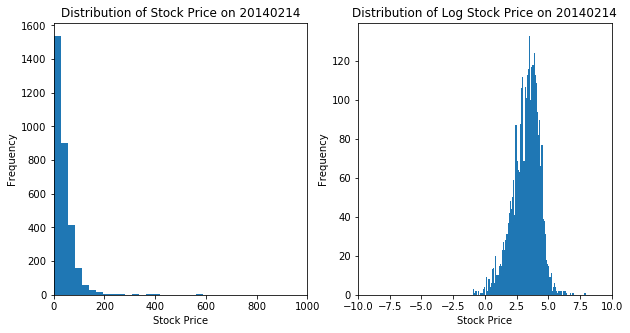
\includegraphics[scale=.35]{stockdis.png}\\ 

\textit{Substantively:} Some concepts are better thought of in terms of ratios than differences. After taking the logged stock prices, we can get the rate of return of stocks by taking the difference of stock prices between two periods.

\textit{The reason to use Z-score feature engineering:}
Investment amounts in our data set are numerical variables. We want to explore whether the investment amounts made by Goldman Sachs will have an impact on the prices of the invested stocks. Since the scales of the tradable shares of different companies are quite different, we should standardize the data to match their scales.

We achieve this by first subtract the data by their empirical mean, and then divide them by their standard deviation of each variable.

\textit{Regression Graphs:}
We tried to explore the long-term effect of the investments made by Goldman Sachs on the stock prices. Therefore, we constructed the regression models using the investment amounts made as independent variables, and stock price changes over the next several quarters as dependent variables. 

\textit{The influence of investments made during 20140214-20140514 on stock price changes in next three quarters:}
For the regression modeling, we used the changes of investment amount during 20140214-20140514 as independent variables, and changes of stock price in 20140214-20140514, 20140514-20140814, 0140814-20141114 as dependent variables respectively. The regression lines and the error plots are shown below:\\ 
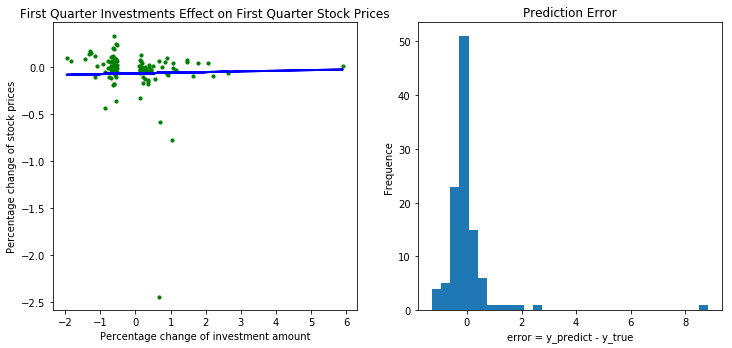
\includegraphics[scale=.32]{log1a.png}\\
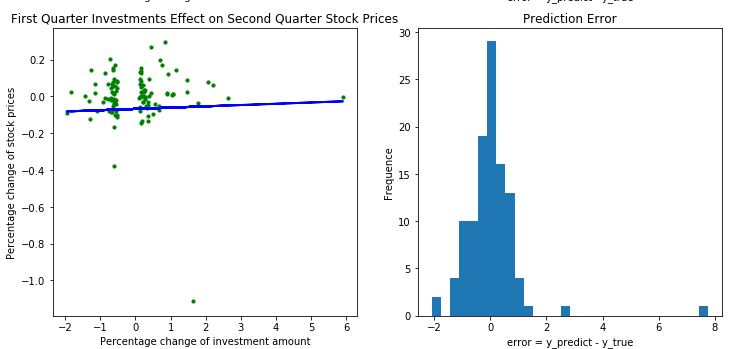
\includegraphics[scale = 0.32]{log1b.png}\\
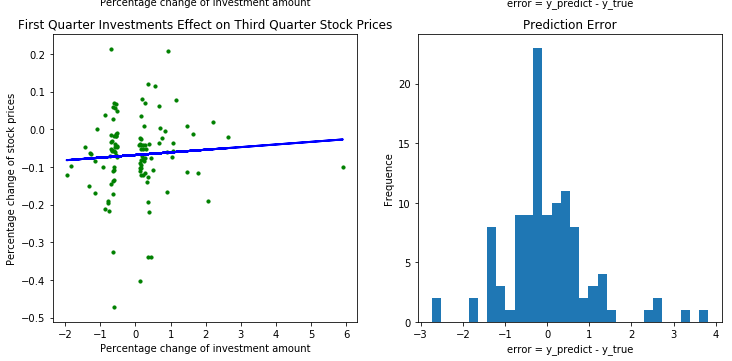
\includegraphics[scale = 0.32]{log1c.png}\\

\textit{The influence of investments during 20140514-20140814 on stock price changes in next two quarters:}
For the regression modeling, we are using the changes of investment amount during 20140514-20140814 as independent variables, and changes of stock price in 20140514-20140814, 0140814-20141114 as dependent variables respectively. The regression lines and error plots are shown below:
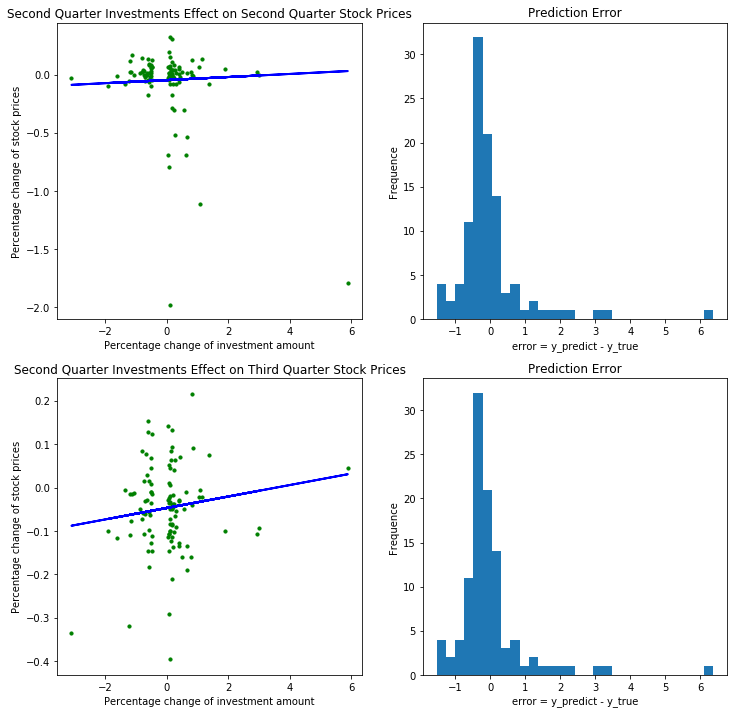
\includegraphics[scale=.32]{logregression2.png}\\[1cm] 

\textit{The influence of investments during 20140814-20141114 on stock price changes in this quarter:}
For the regression modeling, we are using the changes of investment amount during 20140814-20141114 as independent variables, and changes of stock price in 20140814-20141114 as dependent variables respectively. The regression plot is shown below:
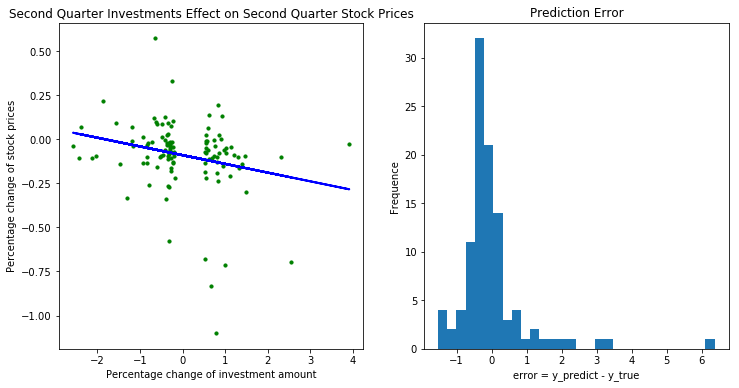
\includegraphics[scale=.32]{logregression3.png}\\[1cm]\\

\textit{Cross Validation Results:}
We split the data set for each regression into training set and test set, and performed cross validation on the data set. The results can be shown as the chart below:
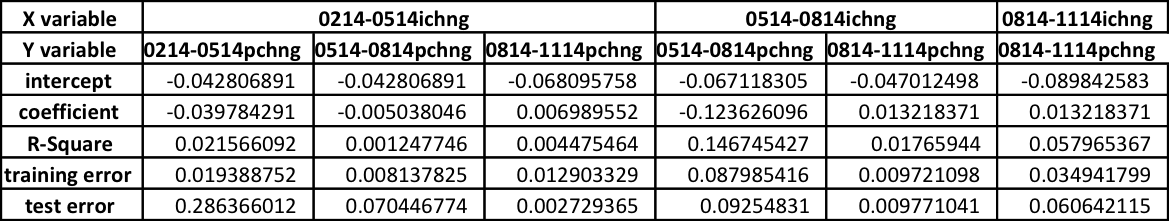
\includegraphics[scale=.44]{logregression.png}\\ \\
From the regression plots and the chart, we can come up with several conclusions:

The investment amounts have a positive correlation with the changes of stock prices if we are using the investment to explain future stock prices. But the correlation is very low. From the plots for investment amounts versus changes of prices in the same quarter, we can see that the correlation is not very significant. Take the investment between 20140214-20140514 as an example, the stock prices within the investment period seems to respond weakly to investment amounts and the correlation is slightly negative. The reasonable premise that the bigger the investment, the bigger the influence on the stock prices is only consistent with the effect of the investment on future quarter. From the plots for investment amounts versus changes of prices in futures quarters, the postive correlation shows up. For example, the changes of stock prices during 20140814-20141114 responded very positively to the investments made one quarter before.

The $R^{2}$ value is low, the changes of price can not be explained well by using the investments made. The test errors in most models are not much higher than the training errors. These model generalize well when new data are used.

The error plots of the regression modeling do not follow a pattern of the normal distribution. From the plots, we can see that the histogram of the errors is right-skewed and has a higher kurtosis, with more extreme points in both sides. We conclude that this is because there are more black swan events in the highly volatile financial market. To deal with it, we used the quantile regression for top quantiles in order to make reasonable prediction for those unexpected extreme events. 


\subsection*{Feature Engineering: \\Polynomial Fit}
We also tried using the same method of linear regression on higher order models via feature engineering. By allowing weights to be placed on our feature as it is raised to different integer values, we can model higher order functions. We found that raising the order of our predictive function to 2 or 3 retained a reasonable proximity to the prediction, while raising it past 6 left us with very variable predictive functions. The large spike in the line is probably due to a localized, noise-based trend upwards that is not corrected for since the data becomes sparser as we move along the x-axis. We can confirm this prediction by looking at the green and red lines, which are the same predictive model run on data from time periods offset by one and two months respectively. Neither of these lines show such a spike in the same area of the x-axis, so it is unlikely that investments in a certain range arbitrarily cause a spike in stock price.

The two graphs show the predictions generated by third and sixth order polynomial functions. As can be seen from the flatness of the first graph, our third order model did not indicate any clear correlation between the amount invested and the stock price of the company invested in. We had similar results for second, and fourth order models, while the fifth order model looked like that of the sixth (the second graph). 



\end{multicols}
\textit{Blue line indicates investments made in first quarter, green are those made in the second, and red are those from the third.}\\
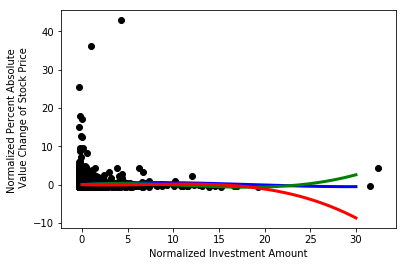
\includegraphics[scale = 0.6]{polyfit.png}
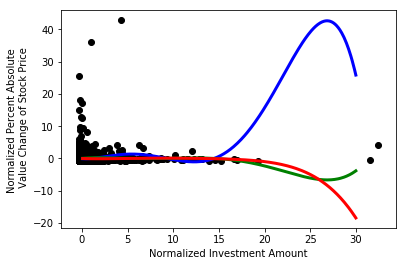
\includegraphics[scale = 0.6]{polyoverfit.png}

\begin{multicols}{2}
[\section*{Quantile Regression}\textit{We estimated the quantile regression model for many quantiles between .05 and .95, and compared best fit line from each of these models to Ordinary Least Squares results.}]

We tried Quantile Regression to model the relationship between the stock price changes and the influential investment. Quantile regression models the response variable (y) for a given quantile (q) conditioned on variable x. In our case, variable x is fixed as the investment amount during 20140214 and 20140514. The Y variable for the three models are namely:  stock price changes between 20140214-20140514, stock price changes between 20140514-20140814, and stock price changes between 20140814-20141114. We intended to see the impact of influential investment over the times.

The following plot on the left is Quantile Regression for corresponding quantities with quantile = [0.5,0.55,0.6,...,0.95]. This plot compares best fit lines for 10 quantile regression models to the least squares fit. Then, the plot on the right is Quantile confidence interval. The dotted black lines form 95\% point-wise confidence band around 10 quantile regression estimates (solid black line). The red lines represent OLS regression results along with their 95\% confidence interval.\\

Quantile plots (investment in the first quarter vs.  stock price change in the first quarter) are as follows:\\
 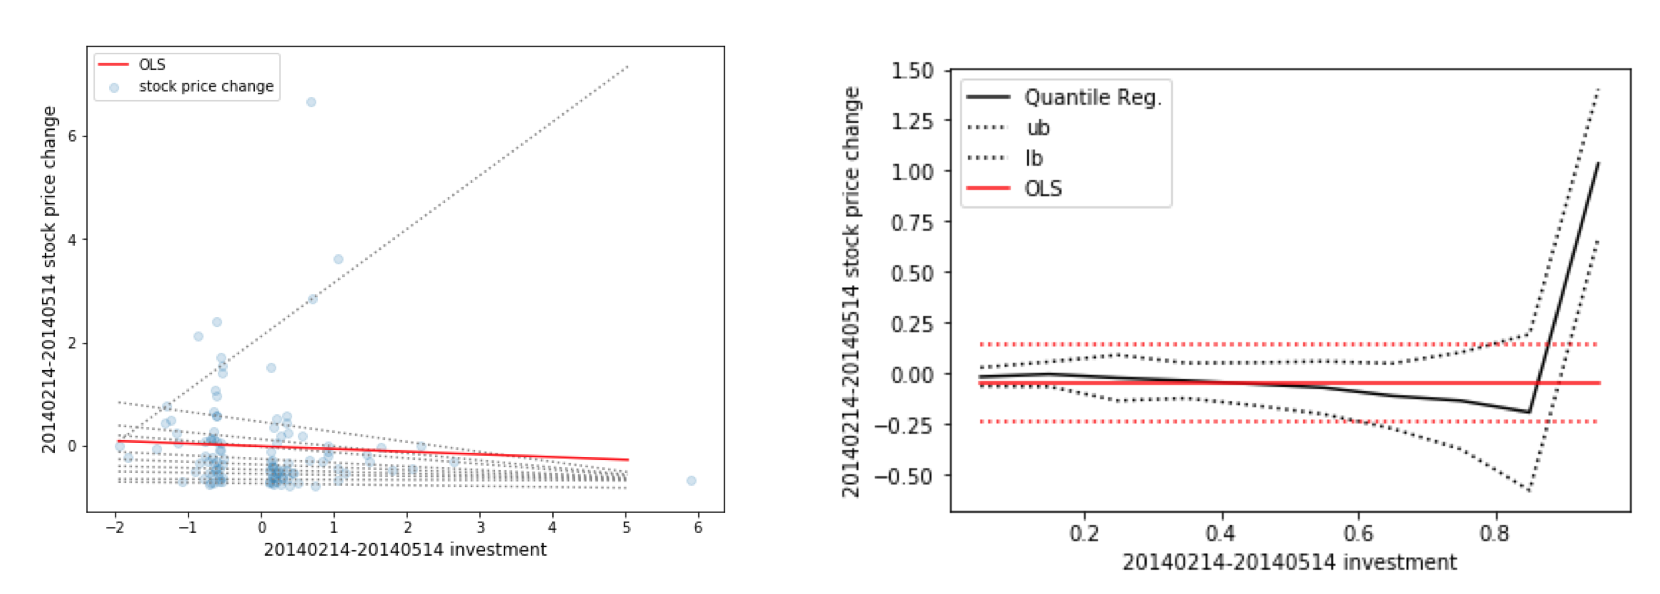
\includegraphics[scale = 0.3]{quantile1.png}\\
Quantile plots (investment in the first quarter vs.  stock price change in the second quarter) are as follows:\\
  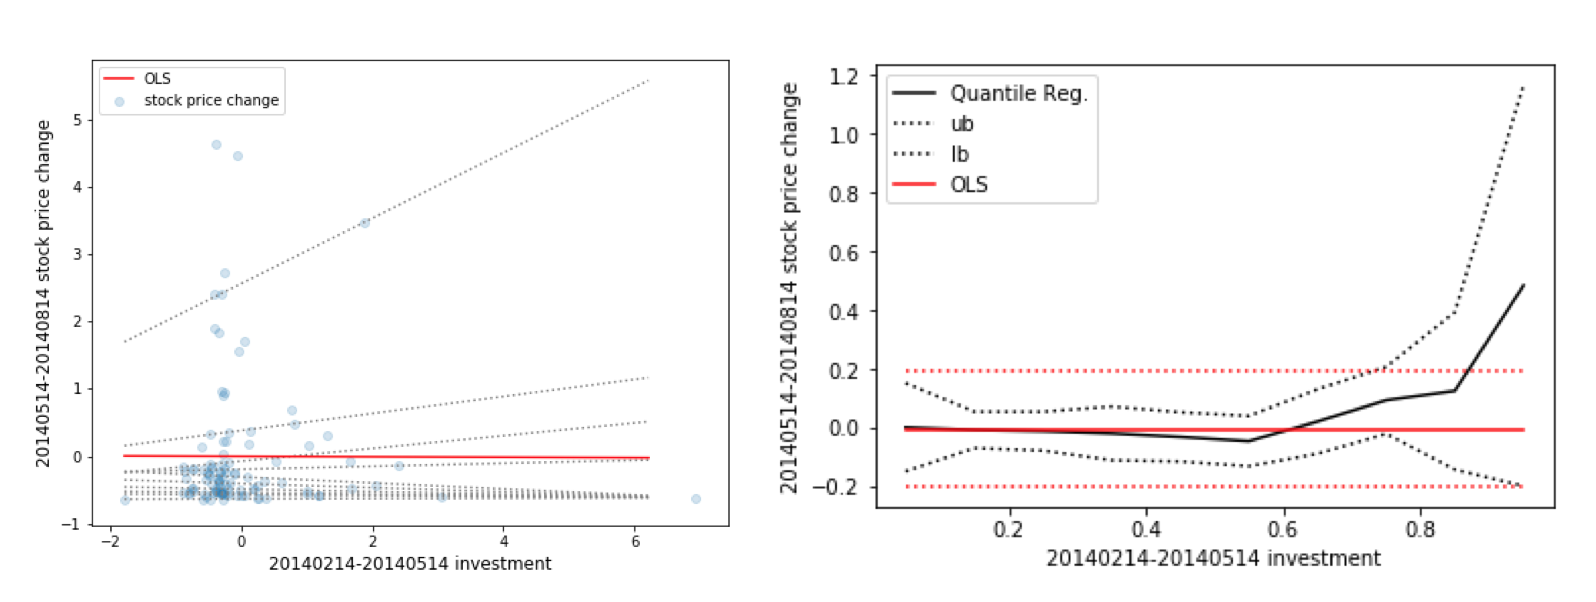
\includegraphics[scale = 0.3]{quantile2.png}\\
Quantile plots (investment in the first quarter vs.  stock price change in the third quarter) are as follows:\\
   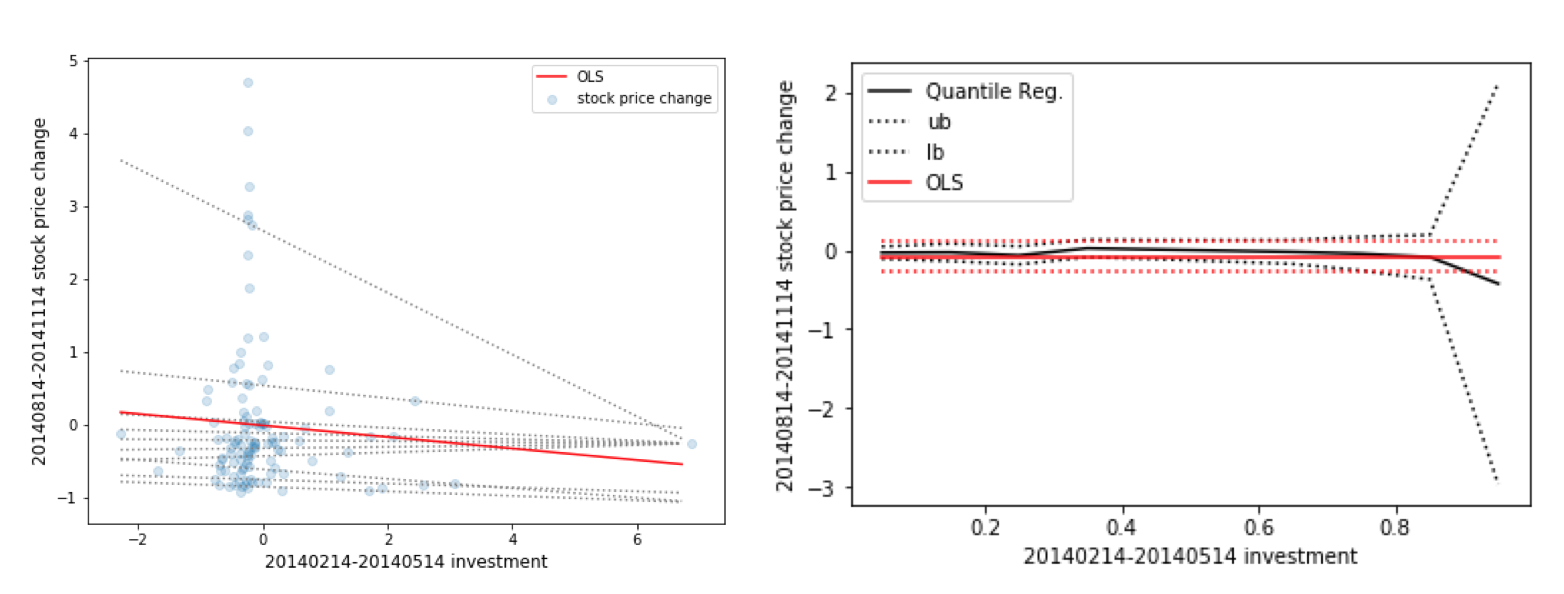
\includegraphics[scale = 0.3]{quantile3.png}\\
 For all the six plots, the higher line indicates the higher percentile.  We made four conclusions from these plots:\\
\begin{enumerate}
\item There is no obvious positive relationship between the influential investment  and the stock performance within the same period.
\item The least squares estimates fit high return stocks poorly (i.e. the OLS lines ignore the performance of most high return stocks).
\item Over the times, the impact of influential investment on stock price in the future seems irrelevant.
\item In most cases, the quantile regression point estimates lie outside the OLS confidence interval, which suggests that the effect of influential investment on stock price may not be constant across the distribution.
\end{enumerate}
 
\end{multicols}

\begin{multicols}{2}
[\section*{Multi-Feature Models and PCA} \textit{If we factor in more variables, we can still tell if influential investment is important by the weights multi-feature models put on this variable}.]

The stock market is a complex entity. Modeling its behavior based on a single factor might be too influenced by other factors to perform well in machine learning. We chose to add other factors we thought might be important for the stocks performance, including the S\&P's average closing value across each month the reports came out (taken from daily closing values), and the price of the companies stock in each quarter (from the calculations mentioned in the Data Cleaning section), in addition to amount invested or divest as we have used in the above modeling techniques. Recognizing that other factors that aren't reflected in our dataset could also lead to large jumps or drops in stock price, we chose to use the RANSAC to get a robust estimator for our data. Based on the investment, S\&P, and price data from February 2014 to May 2014, we predicted the change in stock price by the end of August 2014. 

Next, we performed $R^{2}$ analysis to see how well our model fit the training data. We obtained an $R^{2}$ value that averaged to about 0.45, which falls within the range of significance \footnote{According to Falk and Miller (1992), $R^{2}$ should be $\geq$  0.1 to indicate significance}. 

The graph shows the change in investment amount only, versus the predicted change in stock price. The black dots indicate actual values while the blue line indicates values predicted by the constructed RANSAC model. The second graph below shows the same predictions, but this time versus the change in stock price over the first quarters used to create the model.
\begin{center}
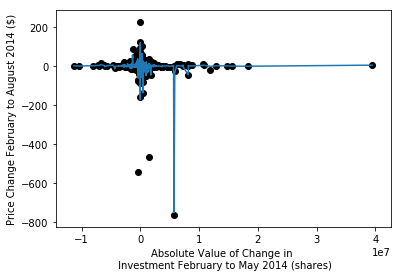
\includegraphics[scale = 0.43]{RansacTrainByAmt.png}
\end{center}

\begin{center}
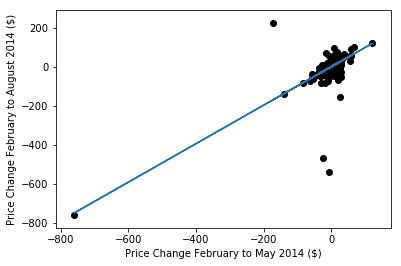
\includegraphics[scale = 0.43]{RansacTrainByPrice.png}
\end{center}
The second graph clearly displays a much more defined line, which implies our model is more dependent on the change in price than the change in investment amount. We confirmed this by looking at the weights generated by the RANSAC model and found that the weight on the price change was 5 orders of magnitude larger than that associated with the change in investment amount. Furthermore, we can see that as the investment approaches zero, the line varies more widely. This makes sense because the smaller the investment, the less effect we expect it to have on the future price of the stock. We used the model generated by the training set on a test set as well and found similar results. 

\begin{center}
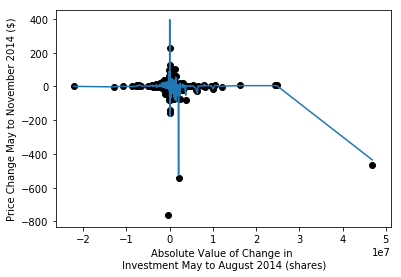
\includegraphics[scale = 0.47]{RansacTestByAmt.png}
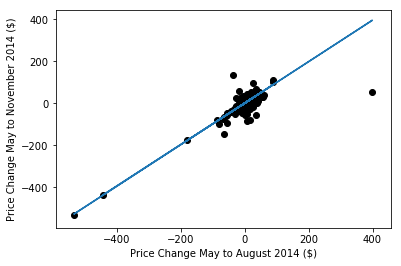
\includegraphics[scale = 0.47]{RansacTestByPrice.png}
\end{center}
Performing PCA on the dataset for all numbers of feature $\leq$ its total number of features, and then conducting $R^{2}$ analysis on the resultant table revealed that any number of features past 2 made negligible changes to performance. We also tried manually omitting the column of our table for change in investment and found that, with the RANSAC method, we achieved very similar performance to when we left it in. 

Thus, we concluded that, for the RANSAC method, there was no significant correlation between the investment amount and the performance of a stock 2 quarters after the investment was made.
\end{multicols}
\begin{multicols}{2}
[\section*{Back Testing}]
After modeling attempts, we leverage back testing to test the performance of the PCA technique. 

For our backtest framework, we applied RANSAC method and used data from February 2014 to May 2014 to train the regression weight, as mentioned in the PCA model. The weights we got are as follows:
\begin{center}
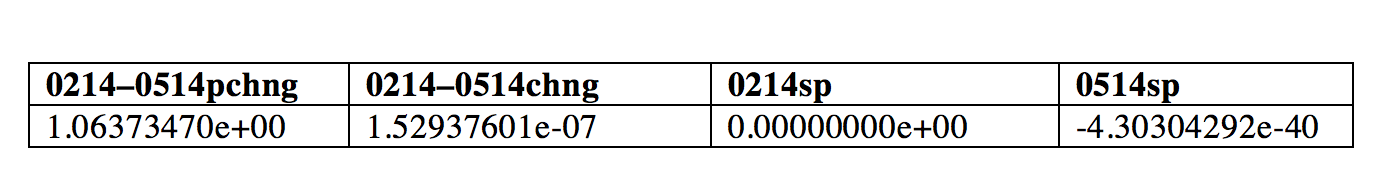
\includegraphics[scale = 0.35]{weight.png}
\end{center}

Then using these trained weights, we tested the results on the quarters of year 2016 and year 2017. We achieved an R-square value of 98.86\%. We discuss the significance of these values in the summary section.


\end{multicols}
\begin{multicols}{2}
[\section*{Summary and Analysis}]
In our project, we tried several different models in order to analyze the power of influential investments on the stock prices. We got some significant results from each attempt:\\

\textit{Log and Z-score:} The models show that the correlation between the investment amount and the changes of stock prices is low and the premise that bigger investment will have larger effect on the price changes does not always hold. Because the error plots of the regression modeling do not follow a pattern of the normal distribution,  We conclude that this is because there are more black swan events in the highly volatile financial market. To deal with it, we used the quantile regression for top quantiles in order to make reasonable prediction for those unexpected extreme events. \\

\textit{Polynomial Fit:} Similar to the Log and Z-score transformations, the polynomial fitting did not increase the apparent fit of the predicted data to the actual data. From these models we deduced that one of the largest problems in fitting the data is that we expect the level of correlation to actually go down the nearer the investment is to zero, and since most of the data points cluster near zero, a trend is hard to determine. However, even at the larger x values, we can see that there is no real trend in the data especially in the higher order graphs since their over-fitting has cause them to be very drastically large in the sparse area of the dataset.\\

\textit{Quantile Regression: }
One thing that we found interesting in plotting the quantiles is that our presupposition that larger investments could have more relevance on stock price seemed to be at least somewhat correct. For the quarter in which the investment was made and, slightly less so, for the quarter after the investment was made,  the normalized values over 0.8 showed a positive trend with quantiles that largely showed a positive trend as well. However, for this project we were mostly interested in the performance in the third quarter after an investment, at which point the quantiles got very large indicating a much looser fit. Additionally, we no longer even found a positive correlation for large values (which could be due to noise, but we cannot assume this as there is no data that supports it). Therefore, using quantile regression showed that there was a correlation between immediate and short term stock prices after a sufficiently large investment, but not for the longer terms we are aiming to look at.
\\

\textit{Multi-Feature Models and PCA:} Since we decided that the investment amount alone could not be used to predict stock price changes with any significant degree of accuracy, we chose to include some other data features and compare their importance to that of investment amount. In our Multi-Feature model, we were able to find a much better fit that performed well on the training data (with an r-squared score in the 40-45\% range), as well as on test data (sets from later in 2014, as well as sets from 2015 and 2016 which had an average r square of 97-99\%). However, when we looked at the weights put on the columns we included, we saw that the weight on the change in amount was much lower than the change in price. If the values in the price change column were much smaller on average than those in the price change column, then the difference in weights could be attributed to scaling the actual values rather than indicating how much the features mattered to the model, but this was not the case. The weight on the price change was much larger than any other weight which led us to believe that the improved performance of this model was mostly due to having the prices in the training data. We supported this conclusion by running the models again on a dataset that did not contain the investment data at all, and found the r-squared values to fall into the same ranges as listed above for all test sets. \\

\textit{Conclusion: } All of our modeling and analysis techniques lead us to the same conclusion; the amount invested in companies by Goldman Sachs does not play a very large role in the third-quarter performance of the stocks of those companies after the investment is made. \\

\textit{Future Work: } 
While we did not find anything to support that large investments in companies by Goldman Sachs affect those companies stock performance multiple quarters after the investment was made, we did find some correlation on shorter terms. From quantile regression, we did find  that very large investments do correlate somewhat with the immediate performance of stocks. This, however, is not of particular interest to us, since quarterly holdings reports only come out at the end of quarters, which is too late to use within that quarter. What is more interesting, is that there might be some correlation between to the price of the stock in the very next quarter after a very large investment. While the correlation is slight, not even registering in Ordinary Least Squares, it might be worth exploring as it could provide an edge in short-term trading.

Another interesting possible expansion on this idea in the future  (that was out of scope for our own project) would be leveraging multiple different extant market modeling services to see these complex models can perform better when given data on actions made by large investment firms on top of the data they already take in. 


\end{multicols}


\end{document}
